\documentclass[english,aspectratio=169,dvipsnames]{beamer}

\usetheme[]{IKRv3}

\usepackage{etoolbox}
\usepackage{parskip}
\usepackage{marvosym}
\usepackage{changepage}
\usepackage{enumitem}
\usepackage{xcolor}
\usepackage{pgfplots}
\usepackage{xcolor}


\usetikzlibrary{positioning}
\usetikzlibrary{calc}
\usetikzlibrary{arrows}
\usetikzlibrary{arrows.meta}
\usetikzlibrary{shapes.geometric}
\usetikzlibrary{fit}
\usetikzlibrary{intersections}
\usetikzlibrary{decorations}
\usetikzlibrary{shadows.blur}
\usetikzlibrary{patterns}
\usetikzlibrary{overlay-beamer-styles}

\selectcolormodel{rgb}

%catpuccin macchiatto colors
\definecolor{rosewatermacchiato}{HTML}{f4dbd6}
\definecolor{flamingomacchiato}{HTML}{f0c6c6}
\definecolor{pinkmacchiato}{HTML}{f5bde6}
\definecolor{mauvemacchiato}{HTML}{c6a0f6}
\definecolor{redmacchiato}{HTML}{ed8796}
\definecolor{maroonmacchiato}{HTML}{ee99a0}
\definecolor{peachmacchiato}{HTML}{f5a97f}
\definecolor{yellowmacchiato}{HTML}{eed49f}
\definecolor{greenmacchiato}{HTML}{a6da95}
\definecolor{tealmacchiato}{HTML}{8bd5ca}
\definecolor{skymacchiato}{HTML}{91d7e3}
\definecolor{sapphiremacchiato}{HTML}{7dc4e4}
\definecolor{bluemacchiato}{HTML}{8aadf4}
\definecolor{lavendermacchiato}{HTML}{b7bdf8}

% \definecolor{text}{HTML}{cad3f5}
% \definecolor{subtext1}{HTML}{b8c0e0}
% \definecolor{subtext0}{HTML}{a5adcb}
% \definecolor{overlay2}{HTML}{939ab7}
% \definecolor{overlay1}{HTML}{8087a2}
% \definecolor{overlay0}{HTML}{6e738d}
% \definecolor{surface2}{HTML}{5b6078}
% \definecolor{surface1}{HTML}{494d64}
% \definecolor{surface0}{HTML}{363a4f}
% \definecolor{base}{HTML}{24273a}
% \definecolor{mantle}{HTML}{1e2030}
% \definecolor{crust}{HTML}{181926}

%catpuccin latte colors
\definecolor{rosewaterlatte}{HTML}{dc8a78}
\definecolor{flamingolattele}{HTML}{dd7878}
\definecolor{pinklatte}{HTML}{ea76cb}
\definecolor{mauvelatte}{HTML}{8839ef}
\definecolor{redlatte}{HTML}{d20f39}
\definecolor{maroonlatte}{HTML}{e64553}
\definecolor{peachlatte}{HTML}{fe640b}
\definecolor{yellowlatte}{HTML}{df8e1d}
\definecolor{greenlatte}{HTML}{40a02b}
\definecolor{teallatte}{HTML}{179299}
\definecolor{sapphirelatte}{HTML}{209fb5}
\definecolor{bluelatte}{HTML}{1e66f5}
\definecolor{skylatte}{HTML}{04a5e5}
\definecolor{lavenderlatte}{HTML}{7287fd}


% policies colors
\newcommand{\kspff}{CornflowerBlue}
\newcommand{\ffksp}{SkyBlue}
\newcommand{\ksplf}{YellowGreen}
\newcommand{\kspbff}{Fuchsia}
\newcommand{\kspbfl}{Thistle}
\newcommand{\kspwff}{BurntOrange}
\newcommand{\kspwfl}{Peach}


\setbeamercolor*{block title example}{fg=black,
bg=greenmacchiato}
\setbeamercolor*{block body example}{fg= black,
bg= IKRBlue!15}


\title{Designing Autoencoder Neural Networks for Efficient IP-Optical Networking}
\subtitle{Master's Thesis}
\date{August 25, 2025} % defaults to \today
\author{Hakan Deli}

% \setbeamertemplate{section in toc} {
%     \hspace{0.5cm}%
%     \tikz[baseline]{
%         %\node[rectangle, fill=white, minimum width = 1mm, minimum height = 1mm] (r1) at (0,0.5) {};%
%         \node[circle, fill = IKRBlue, inner sep = 0.2mm, anchor = center] (n1) at (0,0.11) {\textcolor{white}{\inserttocsectionnumber}};}%
%         \hspace{2mm} \inserttocsection
% }

% \setbeamertemplate{subsection in toc}{\hspace{1.5cm}\inserttocsubsection\\}

\makeatletter
\patchcmd{\beamer@sectionintoc}
  {\vfill}
  {\vskip\itemsep}
  {}
  {}
\makeatother

\makeatletter
\patchcmd{\beamer@subsectionintoc}
  {\vfill}
  {\vspace{-10cm}}
  {}
  {}
\makeatother


\setbeamertemplate{section in toc} {
    \hspace{0.5cm} % Adjust this for consistent indentation across all levels
    \tikz[baseline]{
        \node[circle, fill = IKRBlue, inner sep = 0.2mm, anchor = center] (n1) at (0,0.11) {\textcolor{white}{\inserttocsectionnumber}};
    }%
    \hspace{2mm} \inserttocsection
}


\setbeamertemplate{subsection in toc} {
    \hspace{1.5cm} % Ensure the same amount of indentation as sections
    \tab \inserttocsubsection \\
}

\setlist[itemize]{label=\textcolor{IKRBlue}{\textbullet}}

% \setcounter{tocdepth}{2}

\begin{document}

\begin{frame}[plain]{Outline}
    \vspace{0.4cm}
    \begin{minipage}[t][1cm][t]{\linewidth}
        \setlength{\itemsep}{0cm}
        \setlength{\parskip}{3pt} 
        \tableofcontents[sectionstyle=show,subsectionstyle=show,subsubsectionstyle=hide]
    \end{minipage}
\end{frame}

\breadcrumbson

\section{Introduction}

\begin{frame}{Introduction}{}
    \vspace{0cm}
    \begin{columns}
        \column{0.4\textwidth}
            \begin{adjustwidth}{3mm}{0cm}
                \begin{itemize}
                    \setlength\itemsep{1.5em}
                    \visible<2->{\item growing volume of Internet traffic worldwide}
                    \visible<3->{\item optical communication networks carry the traffic over long distances}
                    \visible<4->{\item must efficiently utilize available resources}
                    \visible<5->{\item network operators must decide on how to route traffic efficiently}
                    \visible<6->{\item decisions highly impact performance}
                \end{itemize}
            \end{adjustwidth}
        \column{0.5\textwidth}
        \only<2-> {
            \begin{figure}[ht]
    	       \begin{adjustwidth}{0cm}{0cm}
        		\centering
        		

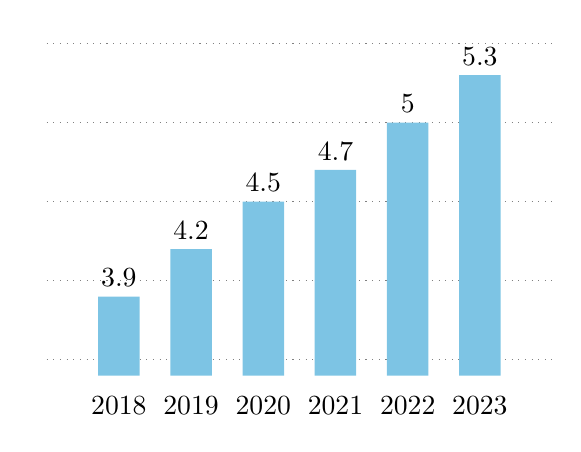
\begin{tikzpicture}
  \begin{axis}[
    ybar,
    bar width=12pt,
    ymin=3.4,
    ymax=5.6,
    ylabel={},
    xlabel={},
    xtick=data, 
    ymajorgrids,
    grid style={dotted,gray},
    y axis line style = {draw = none},
    tick style = {draw=none},
    xticklabel pos = bottom,
    xtick pos = bottom,
    ytick pos = left,
    yticklabels=\empty,
    bar width = 15pt,
    xticklabels={2018,2019,2020,2021,2022,2023},
    nodes near coords,
    nodes near coords align={vertical},
    enlarge x limits=0.2,
    width=8cm, height=6cm
  ]

    \addplot[fill=sapphiremacchiato, draw=none] coordinates {
      (2018,3.9)
      (2019,4.2)
      (2020,4.5)
      (2021,4.7)
      (2022,5.0)
      (2023,5.3)
    };
  \end{axis}
\end{tikzpicture}


        		\vspace{0.2cm}
        		\caption{Cisco annual Internet report showing billions of Internet users}
    	       \end{adjustwidth}
            \end{figure}
        }
    \end{columns}
\end{frame}


\begin{frame}{Introduction}{Motivation: Deep Learning}
    \vspace{0.5cm}
    \begin{adjustwidth}{6mm}{2cm}
                \begin{itemize}
                    \setlength\itemsep{1em}
                    \visible<2->{\item usually standard heuristic methods used for decision finding}
                    \visible<3->{\item advances in machine learning (ML) enable new possibilities}
                    \visible<4->{\item current research only applies reinforcement learning (RL), little to no research on application of deep learning (DL)}
                    \visible<5->{\item DL has the potential to incorporate optimal decisions that can be found previously by an ILP but then be applied in real time by a DNN}
                \end{itemize}
    \end{adjustwidth}

    \begin{center}
    \visible<6-> {
          \begin{minipage}{0.9\linewidth}
              \begin{exampleblock}{First thesis goal}
                derive a DL based decision finding algorithm for network routing
              \end{exampleblock}
          \end{minipage}
    }
   \end{center}

\end{frame}


\begin{frame}{Introduction}{Motivation: Autoencoders}
    \vspace{0.5cm}
    \begin{adjustwidth}{6mm}{2cm}
                \begin{itemize}
                    \setlength\itemsep{1em}
                    \visible<2->{\item are a subfield of DL}
                    \visible<3->{\item can reduce the complexity of neural networks}
                    \visible<4->{\item can act as a unifier for input data of different dimensions}
                    \visible<5->{\item potential to increase performance in decision finding}
                \end{itemize}
    \end{adjustwidth}

    \begin{center}
    \visible<6-> {
          \begin{minipage}{0.9\linewidth}
              \begin{exampleblock}{Second thesis goal}
                examine the use of autoencoders and their effect on performance
              \end{exampleblock}
          \end{minipage}
    }
   \end{center}
\end{frame}


\section{Theoretical Background}


\subsection{Optical Networks and the RSA Problem}

\begin{frame}{Optical Networks and the RSA Problem}{Optical Network Topology}
    \vspace{0.5cm}
	\begin{adjustwidth}{0cm}{0cm}
		\centering
		\tikzstyle{netnode} = [circle, 
					   minimum width = 0.75cm, 
					   minimum height = 0.75cm, 
					   text = black!100, 
					   align=center, 
					   line width = 1, 
					   inner sep = 1mm, 
					   shading=radial, 
					   inner color = sapphiremacchiato!50, 
					   outer color = sapphiremacchiato!100]

\tikzstyle{edge}=[> = stealth, line width = 0.5pt, shorten <= 0mm, shorten >= 0mm]
\tikzstyle{arrow}=[> = stealth, line width = 0.5pt]


\begin{tikzpicture}[x=2cm, y = 2cm]
	
	%Layer42
	\node[netnode, visible on = <2->] (nA) at (-0.53, 1.29) {A};
	\node[netnode, visible on = <2->] (nB) at (-0.35, 0.21) {B};
	\node[netnode, visible on = <4->] (nC) at (-1.39, -0.16) {C};
	\node[netnode, visible on = <4->] (nD) at (0.26, -0.68) {D};
	\node[netnode, visible on = <4->] (nE) at (1.29, -0.76) {E};
	\node[netnode, visible on = <4->] (nF) at (0.72, 0.1) {F};
	
	\draw[edge, <->, visible on = <3->] (nA) -- (nB); 
	\draw[edge, <->, visible on = <4->] (nB) -- (nC);
	\draw[edge, <->, visible on = <4->] (nB) -- (nF);
	\draw[edge, <->, visible on = <4->] (nB) -- (nD);
	\draw[edge, <->, visible on = <4->] (nD) -- (nF);
	\draw[edge, <->, visible on = <4->] (nD) -- (nE);
	\draw[edge, <->, visible on = <4->] (nE) -- (nF);   
	
	\node[align = center, visible on = <2->] (ntext) at (-1.5, 1.1) {node};
	\node[align = center, visible on = <3->] (nlink) at (0.6, 0.85) {optical \\ link};
	
	
	\draw[->, arrow, shorten <= 0.5mm, shorten >= 0.5mm, dashed, red, visible on = <2->] ($ (ntext.east) + (0, 0.03)$) -- ($ (nA.west) + (0, -0.04)$);
	\draw[->, arrow, shorten <= 5mm, shorten >= 1mm, dashed, red, visible on = <3->] ($ (nlink.center) + (0, 0)$) -- (-0.4, 0.7); 
	
	\node[align=center, baseline, visible on = <4->] (t1) at (0, -1.3) {\textbf{Layer42}};
	
	%Mren
	\node[netnode, visible on = <5->] (nAM) at (3.5, 0.29 + 1) {A};
	\node[netnode, visible on = <5->] (nBM) at (4, 0.3) {B};
	\node[netnode, visible on = <5->] (nCM) at (4-1, -0.2) {C};
	\node[netnode, visible on = <5->] (nDM) at (4+1, 0.8) {D};
	\node[netnode, visible on = <5->] (nEM) at (4.5, 0.3 - 1) {E};
	
	\draw[edge, <->, visible on = <5->] (nAM) -- (nBM); 
	\draw[edge, <->, visible on = <5->] (nBM) -- (nCM);
	\draw[edge, <->, visible on = <5->] (nBM) -- (nDM);
	\draw[edge, <->, visible on = <5->] (nBM) -- (nEM);
	
	\node[align=center, baseline, visible on = <5->] (t1) at (4, -1.3) {\textbf{Mren}};
	     
	 
\end{tikzpicture}

	\end{adjustwidth}
\end{frame}

\begin{frame}{Optical Networks and the RSA Problem}{Wavelength-Division Multiplexing and Elastic Optical Networks (EONs)}
	  \vspace{0.0cm}
	\begin{adjustwidth}{0cm}{0cm}
		\centering
		\newcommand{\slotheight}{2cm}
\newcommand{\slotwidth}{2mm}
\newcommand{\numchannels}{10}
\newcommand{\fsperchannel}{5}
\newcommand{\lw}{1pt}

\tikzstyle{slot} = [draw = black,
					minimum width = \slotwidth, 
				    minimum height = \slotheight, 
					text = black!100, 
					anchor = west, 
					line width = \lw,
					inner sep = 0mm]
					
\tikzstyle{legendtext} = [text = black,
						  anchor = north, 
						  align = center, 
						  inner sep = 0mm,
						  font = \scriptsize]

\tikzstyle{arrow}=[> = stealth, line width = 0.5pt, dashed, red]

%{coordinate}{amount of fs}{color}{height}
\newcommand{\spectrum}[4]{%
	\path (#1) coordinate (start);
	\fill[fill opacity=0.5, fill=#3]
	($(start) + (0, \lw)$)
	-- ($ (start) + (#2*0.5*\slotwidth-0.5*\lw,\lw) $)
	arc[start angle=0, end angle=180, x radius=#2*0.5*\slotwidth-0.5*\lw, y radius=#4-\lw]
	-- cycle;
}

\newcommand{\oneslot}[2]{
	\spectrum{#1}{1}{blue}{#2}
}

\newcommand{\twoslot}[2]{
	\spectrum{#1}{2}{blue}{#2}
}

\newcommand{\threeslot}[2]{
	\spectrum{#1}{3}{violet}{#2}
}

\newcommand{\fourslot}[2]{
	\spectrum{#1}{4}{ForestGreen}{#2}
}

\newcommand{\fiveslot}[2]{
	\spectrum{#1}{5}{red}{#2}
}

\newcommand{\twelveslot}[2]{
	\spectrum{#1}{12}{orange}{#2}
}



%\tikzstyle{edge}=[> = stealth, line width = 0.5pt, shorten <= 0mm, shorten >= 0mm]
%\tikzstyle{arrow}=[> = stealth, line width = 0.5pt]

\begin{tikzpicture}[x=1cm, y=1cm]
	
	
	%WDM

    \node[draw = black, 
          minimum width = 10*\slotwidth*\fsperchannel, 
		   minimum height = \slotheight, 
		   text = black!100, 
		   anchor = west, 
		   line width = \lw,
		   inner sep = 0mm, visible on = <2>] (startbox) at (0, -0.4) {};
    
	\foreach \i in {1,...,\numchannels}{
		\pgfmathtruncatemacro{\j}{\i-1}
		\node[slot, minimum width = \slotwidth*\fsperchannel, visible on = <3->] (wdm\i) at (\j*\slotwidth*\fsperchannel, -0.4) {};
	}
	
	\node[text = black, left = 0.5cm of wdm1.west, anchor = east, visible on = <3->] (wdmtext) {WDM};
	
	%WDM spectras
	\visible<5->{\threeslot{wdm1.south}{0.98*\slotheight}}
	\visible<5->{\fiveslot{wdm2.south}{0.98*\slotheight}}
	\visible<5->{\twoslot{wdm3.south}{0.98*\slotheight}}
	\visible<5->{\fourslot{wdm7.south}{0.98*\slotheight}}
	\visible<5->{\fourslot{wdm8.south}{0.98*\slotheight}}
	\visible<5->{\twoslot{wdm9.south}{0.98*\slotheight}}
	
	%cut the top off
%	\draw[-, draw=white, line width=1mm, align=center] (wdm1.north west) -- (wdm\numchannels.north east);	
	
	%EON
    
	\pgfmathtruncatemacro{\amount}{\numchannels*\fsperchannel}
	\foreach \i in {1,...,\amount}{
		\pgfmathtruncatemacro{\j}{\i-1}
		\node[slot, minimum width = \slotwidth, draw = black!20, line width = 0.5*\lw, visible on = <7->] (fs\i) at (\j*\slotwidth+0.125*\lw, -3.4) {};
	}
	
	\node[text = black, left = 0.5cm+0.5*\lw of fs1.west, anchor = east, visible on = <7->] (eontext) {EON};
	
	%draw eon channels by hand	
	\foreach \ns/\nend in  {fs1/fs3,
						    fs4/fs8,
	                        fs9/fs10,
	                        fs11/fs22,
	                        fs23/fs30,
	                        fs31/fs34,
	                        fs35/fs38,
	                        fs39/fs40,
	                        fs41/fs50}{

	\draw[-, draw=black, line width=\lw, align=center, visible on = <9->] (\ns.north west)++(0.25*\lw,0) -- ($(\ns.south west)+(0.25*\lw, 0.5*\lw)$) -- ($(\nend.south east) + (-0.25*\lw, 0.5*\lw)$) -- ($(\nend.north east)+(-0.25*\lw,0)$);
	                        
	}

	%eon spectra
	\visible<9->{\threeslot{fs2.south}{0.98*\slotheight}}
	\visible<9->{\fiveslot{fs6.south}{0.98*\slotheight}}
	\visible<9->{\twoslot{fs9.south east}{0.98*\slotheight}}
	\visible<9->{\twelveslot{fs16.south east}{0.98*\slotheight}}
	\visible<9->{\fourslot{fs32.south east}{0.98*\slotheight}}
	\visible<9->{\fourslot{fs36.south east}{0.98*\slotheight}}
	\visible<9->{\twoslot{fs39.south east}{0.98*\slotheight}}
	
	%legend
	\foreach \y in {1,2,...,5}{
		\node[inner sep = 0mm, anchor = center, visible on = <5->] (l\y) at (12,-1.3*\y+1.8) {};
	}
	
	\node[legendtext, below = 1pt of l1.south, visible on = <5->] {25 GHz};
	\node[legendtext, below = 1pt of l2.south, visible on = <5->] {37.5 GHz};
	\node[legendtext, below = 1pt of l3.south, visible on = <5->] {50 GHz};
	\node[legendtext, below = 1pt of l4.south, visible on = <5->] {62.5 GHz};
	\node[legendtext, below = 1pt of l5.south, visible on = <5->] {150 GHz};
	
	\visible<5->{\twoslot{l1.center}{0.2*\slotheight}}
	\visible<5->{\threeslot{l2.center}{0.2*\slotheight}}
	\visible<5->{\fourslot{l3.center}{0.2*\slotheight}}
	\visible<5->{\fiveslot{l4.center}{0.2*\slotheight}}
	\visible<5->{\twelveslot{l5.center}{0.2*\slotheight}}

    \node[draw = black, 
          minimum width = 10*\slotwidth*\fsperchannel, 
		   minimum height = \slotheight, 
		   text = black!100, 
		   anchor = west, 
		   line width = \lw,
		   inner sep = 0mm, visible on = <6->] (startboxeon) at (-0.005, -3.4) {};
    
	%highlight one frequency slot and one optical channel
	\node[slot, minimum width = \slotwidth, draw = red, line width = 1.25*\lw, left = 0cm of fs44.west, anchor = west, pattern = north east lines, pattern color = red, visible on = <8->] (fsred) {};
	\node[slot, minimum width = \slotwidth*\fsperchannel, draw = red, line width = 1.25*\lw, left = 0cm of wdm5.west, anchor = west, pattern = north east lines, pattern color = red, visible on = <4->] (wdmred) {};
	
	%add arrows and explanatory text
	\node[legendtext, font = \normalsize, visible on = <4->] (wdmarrowtext) at (4.5,-1.55) {\small one WDM channel};
	\node[legendtext, font = \normalsize, align = center, visible on = <8->] (eonarrowtext) at (8.71,-4.7) {\small one FS \\ \small (12.5 GHz)};
	
	\draw[->, draw = gray, > = stealth, line width = 0.5pt, visible on = <2->] (-0.1,-1.9) -- (10.2,-1.9) node[right] {\textcolor{gray}{$\lambda$}};
    
	
	
\end{tikzpicture}
	\end{adjustwidth}
\end{frame}

\begin{frame}{Optical Networks and the RSA Problem}{}
	\begin{textblock}{5}(1, 1.4)
        \tikzstyle{netnode} = [circle, 
					   minimum width = 0.25cm, 
					   minimum height = 0.25cm, 
					   text = black!100, 
					   align=center, 
					   line width = 1, 
					   inner sep = 0.5mm, 
					   shading=radial, 
					   inner color = sapphiremacchiato!50, 
					   outer color = sapphiremacchiato!100]

\tikzstyle{edge}=[> = stealth, line width = 0.3pt, shorten <= 0mm, shorten >= 0mm]


\newcommand{\slotheight}{1.2cm}
\newcommand{\slotwidth}{1mm}
\newcommand{\numchannels}{10}
\newcommand{\fsperchannel}{5}
\newcommand{\lw}{1pt}

\tikzstyle{slot} = [draw = black,
					minimum width = \slotwidth, 
				    minimum height = \slotheight, 
					text = black!100, 
					anchor = west, 
					line width = \lw,
					inner sep = 0mm]

    
\begin{tikzpicture}

    %background rectangles
    \node[rectangle, fill = IKRBlue!20, minimum width = 14cm, minimum height = 6.9cm, rounded corners = 5pt, anchor = north west, visible on = <2->] at (0,0) {};
    \node[rectangle, fill = white, minimum width = 6cm, minimum height = 3cm, rounded corners = 5pt, anchor = north west, visible on = <3->] at (0.5,-0.8) {};
    \node[rectangle, fill = white, minimum width = 6cm, minimum height = 3cm, rounded corners = 5pt, anchor = north west, visible on = <5->] at (7.5,-0.8) {};

    %plus
    \begin{scope}[shift={(7cm,-2.3cm)}, visible on = <5->]
          \def\arm{0.05}   % half-width of arms
          \def\len{0.2}     % half-length of plus arms
          % Draw filled plus shape centered at (0,0)
          \filldraw[IKRBlue]
          (-\arm, -\len) rectangle (\arm, \len)  % vertical bar
          (-\len, -\arm) rectangle (\len, \arm); % horizontal bar
    \end{scope}

    %text
    \node[anchor = west, visible on = <2->] at (0.2, -0.45) {\textbf{R}outing and \textbf{S}pectrum \textbf{A}ssignment Problem};
    \node[anchor = center, align = center, visible on = <3->] at (3.4, -4.15) {Route};
    \node[anchor = center, align = center, visible on = <5->] at (10.5, -4.15) {Spectrum};

    %layer42
    \begin{scope}[x=1.3cm, y=1.1cm, shift={(3.5cm, -2.6cm)}]
    
        %vanilla
        \node[netnode, visible on = <3->] (nA) at (-0.53, 1.29) {\small A};
        \node[netnode, visible on = <3>] (nB) at (-0.35, 0.21) {\small B};
        \node[netnode, visible on = <3->] (nC) at (-1.39, -0.16) {\small C};
        \node[netnode, visible on = <3->] (nD) at (0.26, -0.68) {\small D};
        \node[netnode, visible on = <3->] (nE) at (1.29, -0.76) {\small E};
        \node[netnode, visible on = <3>] (nF) at (0.72, 0.1) {\small F};
        
        \draw[edge, <->, visible on = <3>] (nA) -- (nB); 
        \draw[edge, <->, visible on = <3>] (nB) -- (nC);
        \draw[edge, <->, visible on = <3>] (nB) -- (nF);
        \draw[edge, <->, visible on = <3>] (nB) -- (nD);
        \draw[edge, <->, visible on = <3>] (nD) -- (nF);
        \draw[edge, <->, visible on = <3>] (nD) -- (nE);
        \draw[edge, <->, visible on = <3>] (nE) -- (nF);  
    
        %scenario
        \node[  netnode, 
                inner color = red!20, 
				outer color = red!70,
                visible on = <4->] (nBs) at (-0.35, 0.21) {\small B};

        \node[  netnode, 
                inner color = red!20, 
				outer color = red!70,
                visible on = <4->] (nFs) at (0.72, 0.1) {\small F};

        \draw[edge, <->, opacity = 0.3, visible on = <4->] (nA) -- (nB); 
        \draw[edge, <->, opacity = 0.3, visible on = <4->] (nB) -- (nC);
        \draw[edge, draw = ForestGreen, ->, visible on = <4->] (nB) -- (nF);
        \draw[edge, draw = Orchid, ->, visible on = <4->] (nB) -- (nD);
        \draw[edge, draw = Orchid, ->, visible on = <4->] (nD) -- (nF);
        \draw[edge, <->, opacity = 0.3, visible on = <4->] (nD) -- (nE);
        \draw[edge, <->, opacity = 0.3, visible on = <4->] (nE) -- (nF); 
        
    \end{scope}

    %spectrum

    \begin{scope}[shift={(8cm,-2.5cm)}]
    
        %EON
    	\pgfmathtruncatemacro{\amount}{\numchannels*\fsperchannel}
    	\foreach \i in {1,...,\amount}{
    		\pgfmathtruncatemacro{\j}{\i-1}
    		\node[slot, minimum width = \slotwidth, draw = black!20, line width = 0.5*\lw, visible on = <5->] (fs\i) at (\j*\slotwidth+0.125*\lw, 0) {};
    	}
    	
    	%draw eon channels by hand	
    	\foreach \ns/\nend in  {fs1/fs3,
    						    fs7/fs10,
    	                        fs23/fs28,
    	                        fs41/fs50}{
    
    	\fill[fill=red, opacity = 0.5, visible on = <5->] (\ns.north west)++(0.25*\lw,0) -- ($(\ns.south west)+(0.25*\lw, 0.5*\lw)$) -- ($(\nend.south east) + (-0.25*\lw, 0.5*\lw)$) -- ($(\nend.north east)+(-0.25*\lw,0)$) -- cycle;
    	                        
    	}
    
        \node[draw = black, 
              minimum width = 10*\slotwidth*\fsperchannel, 
    		   minimum height = \slotheight, 
    		   text = black!100, 
    		   anchor = west, 
    		   line width = \lw,
    		   inner sep = 0mm, visible on = <5->] (startboxeon) at (-0.005, 0) {};

        \draw[->, line width = 1pt, draw = red, > = Stealth , shorten >= 0.5mm, visible on = <6->] ($(fs13.north) + (0, 0.6)$) -- (fs13.north);
    
    \end{scope}


    % constraints
    \node[rectangle, fill = IKRBlue!5, minimum width = 4.4cm, minimum height = 2cm, rounded corners = 5pt, anchor = north west, align = center, text height = 1cm, text depth = 0.5cm, visible on = <7->] at (0.2,-4.7) {FS $\leftrightarrow$ optical channel};
    \node[rectangle, fill = IKRBlue!5, minimum width = 4.4cm, minimum height = 2cm, rounded corners = 5pt, anchor = north west, align = center, text height = 1cm, text depth = 0.5cm, visible on = <8->] at (4.8,-4.7) {no wavelength conversion};
    \node[rectangle, fill = IKRBlue!5, minimum width = 4.4cm, minimum height = 2cm, rounded corners = 5pt, anchor = north west, align = center, text height = 1cm, text depth = 0cm, visible on = <9->] at (9.4,-4.7) {assigned FSs are \\ adjacent};

    \node[anchor = center, align = center, visible on = <7->] at (2.4, -5.2) {\textbf{Capacity}};
    \node[anchor = center, align = center, visible on = <8->] at (7, -5.2) {\textbf{Continuity}};
    \node[anchor = center, align = center, visible on = <9->] at (11.6, -5.2) {\textbf{Contiguity}};
    
 
\end{tikzpicture}
					
    \end{textblock}
\end{frame}


\begin{frame}{Optical Networks and the RSA Problem}{Heuristic Two-Step Approaches}
	\begin{textblock}{5}(0.6, 1.9)
        \tikzstyle{netnode} = [circle, 
					   minimum width = 0.15cm, 
					   minimum height = 0.15cm, 
					   text = black!100, 
					   align=center, 
					   line width = 1, 
					   inner sep = 0.3mm, 
					   shading=radial, 
					   inner color = sapphiremacchiato!50, 
					   outer color = sapphiremacchiato!100]

\tikzstyle{netnodebig} = [circle, 
					   minimum width = 0.25cm, 
					   minimum height = 0.25cm, 
					   text = black!100, 
					   align=center, 
					   line width = 1, 
					   inner sep = 0.5mm, 
					   shading=radial, 
					   inner color = sapphiremacchiato!50, 
					   outer color = sapphiremacchiato!100]

\tikzstyle{edge}=[> = stealth, line width = 0.2pt, shorten <= 0mm, shorten >= 0mm]


\newcommand{\slotheight}{1.6cm}
\newcommand{\slotwidth}{1.5mm}
\newcommand{\numchannels}{10}
\newcommand{\fsperchannel}{5}
\newcommand{\lw}{1pt}

\tikzstyle{slot} = [draw = black,
					minimum width = \slotwidth,
				    minimum height = \slotheight, 
					text = black!100,
					anchor = west,
					line width = \lw,
					inner sep = 0mm]

    
\begin{tikzpicture}

    %background rectangles
    \node[rectangle, fill = IKRBlue!20, minimum width = 14.7cm, minimum height = 6.5cm, rounded corners = 5pt, anchor = north west, visible on = <1->] at (0,0) {};
    \node[rectangle, fill = white, minimum width = 5.3cm, minimum height = 5cm, rounded corners = 5pt, anchor = north west, visible on = <2->] at (0.5,-0.8) {};
    \node[rectangle, fill = white, minimum width = 8cm, minimum height = 5cm, rounded corners = 5pt, anchor = north west, visible on = <4->] at (6.2,-0.8) {};

    %text
    \foreach \heur/\v in {  FF/6,
                            LF/7,
                            BFF/8,
                            BFL/9,
                            WFF/10,
                            WFL/11
                         } \node[anchor = west, visible on = <\v>] at (0.1, -0.4) {Policy $\pi_{\text{KSP-\heur}}$};
    \node[anchor = center, align = center, visible on = <3->] at (3.1, -6.15) {$K$-shortest paths (KSPs)};
    \node[anchor = center, align = center, visible on = <4->] at (10.2, -6.15) {heuristic slot selection};

    %layer42
    \begin{scope}[x=0.8cm, y=0.7cm, shift={(3.15cm, -2.1cm)}]
    
        %vanilla
        \node[netnode, inner color = red!20, outer color = red!70, visible on = <2->] (nA) at (-0.53, 1.29) {\footnotesize A};
        \node[netnode, visible on = <2->] (nB) at (-0.35, 0.21) {\footnotesize B};
        \node[netnode, visible on = <2->] (nC) at (-1.39, -0.16) {\footnotesize C};
        \node[netnode, visible on = <2->] (nD) at (0.26, -0.68) {\footnotesize D};
        \node[netnode, inner color = red!20, outer color = red!70, visible on = <2->] (nE) at (1.29, -0.76) {\footnotesize E};
        \node[netnode, visible on = <2->] (nF) at (0.72, 0.1) {\footnotesize F};
        
        \draw[edge, <->, visible on = <2-3>] (nA) -- (nB); 
        \draw[edge, <->, visible on = <2->] (nB) -- (nC);
        \draw[edge, <->, visible on = <2-3>] (nB) -- (nF);
        \draw[edge, <->, visible on = <2->] (nB) -- (nD);
        \draw[edge, <->, visible on = <2->] (nD) -- (nF);
        \draw[edge, <->, visible on = <2->] (nD) -- (nE);
        \draw[edge, <->, visible on = <2-3>] (nE) -- (nF);  

        \draw[edge, color = red, ->, visible on = <4->] (nA) -- (nB); 
        \draw[edge, color = red, ->, visible on = <4->] (nB) -- (nF); 
        \draw[edge, color = red, ->, visible on = <4->] (nF) -- (nE); 
        
    \end{scope}

    %ksps

    \begin{scope}[x=0.9cm, y= 0.6cm, shift={(-0.2cm,-1cm)}]
        \foreach \x/\y/\lbl/\i in { 1.5/-4/{1.}/0, 2/-4/A/1, 3/-4/B/2, 4/-4/F/3, 5/-4/E/4,%
                                    1.5/-5/{2.}/0, 2/-5/A/5, 3/-5/B/6, 4/-5/D/7, 5/-5/E/8,
                                    1.5/-6/{3.}/0, 2/-6/A/9, 3/-6/B/10, 4/-6/F/11, 5/-6/D/12, 6/-6/E/13,
                                    1.5/-7/{4.}/0, 2/-7/A/14, 3/-7/B/15, 4/-7/D/16, 5/-7/F/17, 6/-7/E/18} {
                                    \node[visible on = <3->] (n\i) at (\x, \y) {\small \lbl};
                                }
        \foreach \x/\y/\lbl/\i in { 1.5/-4/{1.}/0, 2/-4/A/1, 3/-4/B/2, 4/-4/F/3, 5/-4/E/4} 
                                    {
                                    \node[visible on = <4->] (n\i) at (\x, \y) {\small \textcolor{red}{\lbl}};
                                    }
    \end{scope}
    \foreach \i/\j in { 1/2, 2/3, 3/4, 
                        5/6, 6/7, 7/8, 
                        9/10, 10/11, 11/12, 12/13,
                        14/15, 15/16, 16/17, 17/18}
                        \draw[->, > = Stealth, line width = 0.2pt, visible on = <3->] (n\i) -- (n\j);
    
    \foreach \i/\j in {1/2, 2/3, 3/4} \draw[->, > = Stealth, draw = red, line width = 0.2pt, visible on = <4->] (n\i) -- (n\j);


    %spectrum

    \begin{scope}[shift={(6.45cm, -4.5cm)}]
    
        % EON
    	\pgfmathtruncatemacro{\amount}{\numchannels*\fsperchannel}
    	\foreach \i in {1,...,\amount}{
    		\pgfmathtruncatemacro{\j}{\i-1}
    		\node[slot, minimum width = \slotwidth, draw = black!20, line width = 0.5*\lw, visible on = <4->] (fs\i) at (\j*\slotwidth+0.125*\lw, 0) {};
    	}
    	
    	% draw eon channels by hand	
    	\foreach \ns/\nend in  {fs1/fs3,
    						    fs13/fs18,
    	                        fs26/fs29,
    	                        fs45/fs48}{
    
    	\fill[fill=red, opacity = 0.5, visible on = <4->] (\ns.north west)++(0.25*\lw,0) -- ($(\ns.south west)+(0.25*\lw, 0.5*\lw)$) -- ($(\nend.south east) + (-0.25*\lw, 0.5*\lw)$) -- ($(\nend.north east)+(-0.25*\lw,0)$) -- cycle;
    	                        
    	}

        % heuristics 	
    	
        % allocations
        \foreach \ns/\nend/\strat/\v in  {  fs4/fs6/\kspff/6,
                                            fs42/fs44/\kspff/7,
    	                                      fs19/fs21/\kspff/8,
                                            fs23/fs25/\kspff/9,
                                            fs30/fs32/\kspff/10,
                                            fs42/fs44/\kspff/11} {
    
    	\fill[fill=\strat, opacity = 0.5, visible on = <\v>] (\ns.north west)++(0.25*\lw,0) -- ($(\ns.south west)+(0.25*\lw, 0.5*\lw)$) -- ($(\nend.south east) + (-0.25*\lw, 0.5*\lw)$) -- ($(\nend.north east)+(-0.25*\lw,0)$) -- cycle;
    	                        
    	}


        % Text
        \foreach \heurtext/\v in  {   {\textbf{F}irst \textbf{F}it}/6,
    	                               {\textbf{L}ast \textbf{F}it}/7,
                                      {\textbf{B}est \textbf{F}it \textbf{F}irst}/8,
                                      {\textbf{B}est \textbf{F}it \textbf{L}ast}/9,
                                      {\textbf{W}orst \textbf{F}it \textbf{F}irst}/10,
                                      {\textbf{W}orst \textbf{F}it \textbf{L}ast}/11}{

            \node[align = center, visible on = <\v>] at (3, 2.4) {\heurtext};

        }


        % sample block
        \pgfmathtruncatemacro{\amount}{3}
    	\foreach \i in {1,...,\amount}{
    		\pgfmathtruncatemacro{\j}{\i-1}
    		\node[slot, minimum width = \slotwidth, draw = black!20, line width = 0.5*\lw, visible on = <5->] (fse\i) at (\j*\slotwidth+0.125*\lw+5cm, 2.4) {};
    	}
        \fill[fill=\kspff, opacity = 0.5, visible on = <5->] (fse1.north west)++(0.25*\lw,0) -- ($(fse1.south west)+(0.25*\lw, 0.5*\lw)$) -- ($(fse3.south east) + (-0.25*\lw, 0.5*\lw)$) -- ($(fse3.north east)+(-0.25*\lw,0)$) -- cycle;

        % arrows
        \foreach \s/\v in { fs5/6,
                            fs20/8,
                            fs24/9,
                            fs31/10,
                            fs43/11,
                            fs43/7
                            } {
            \draw[-{Stealth[length=2mm, width=1mm]}, line width = 0.5pt, draw = black, visible on = <\v>] ($(fse2.south) + (0, -0.05)$) -- ($(\s.north) + (0, 0.05)$);
        }

        % % FS numbers
        % \node[below = 0mm of fs1, align = center, visible on = <5->] {\tiny $1$};
        % \node[below = 0mm of fs50, align = center, visible on = <5->] {\tiny $50$};
    
    \end{scope}

    % Z1: I I I I _ I _ I I I
    % Z2: W _ W _ _ _ W _ W W
    % Z3: I _ I _ I _ I _ I _
    % Z4: I links
    % Z5: I links (rigged)
 
\end{tikzpicture}
					
    \end{textblock}
\end{frame}


\subsection{Deep Learning}

\begin{frame}{Deep Learning}{}
	
\end{frame}


\begin{frame}{Deep Learning}{Deep Neural Networks (DNNs)}
            
\end{frame}


\subsection{Autoencoders}

\begin{frame}{Autoencoders}{}
	
\end{frame}


\section{Environment Setup}


\subsection{Network State}

\begin{frame}{Environment Setup}{}
	
\end{frame}


\subsection{The RSA Episode}



\section{DL Policy for RSA Problem}

\subsection{Basic Policy}

\begin{frame}{Basic DNNs for RSA Problem}{Processing Pipeline}
	
\end{frame}


\subsection{Policymix Approach}

\begin{frame}{Policymix for RSA Problem}{}
	
\end{frame}


\subsection{Autoencoder Policy}

\begin{frame}{Autoencoder for RSA Problem}{}
	 
\end{frame}



\section{Conclusion and Outlook}

\begin{frame}{Conclusion and Outlook}{}
	 
\end{frame}

\end{document}
